\section{Funktionsumfang}
Im Folgenden beschreiben wir den Funktionsumfang des Self-Service-Terminal sowie das erwartete Verhalten der Anwendung bei Ausführung besagter Funktionen. Der Übersichtlichkeit halber unterscheiden wir in Funktionen der Administratorensicht und der Kundensicht. Mit Kundensicht meinen wir in diesem Kontext die Benutzeroberfläche für die Kunden in der Filiale; mit Administratorensicht ist die Benutzeroberfläche für die Administratoren des Self-Service-Terminal gemeint.\\

\subsection{Administrationssicht}


\subsubsection{Benutzer} Benutzer können angelegt und gelöscht werden. Zu jedem Benutzer können Benutzername, Vorname, Nachname, E-Mail, Passwort, Berechtigungen, Gruppenzugehörigkeit und Login-Daten gespeichert werden (Abbildung 1).

\begin{figure}[htp]
    \centering
    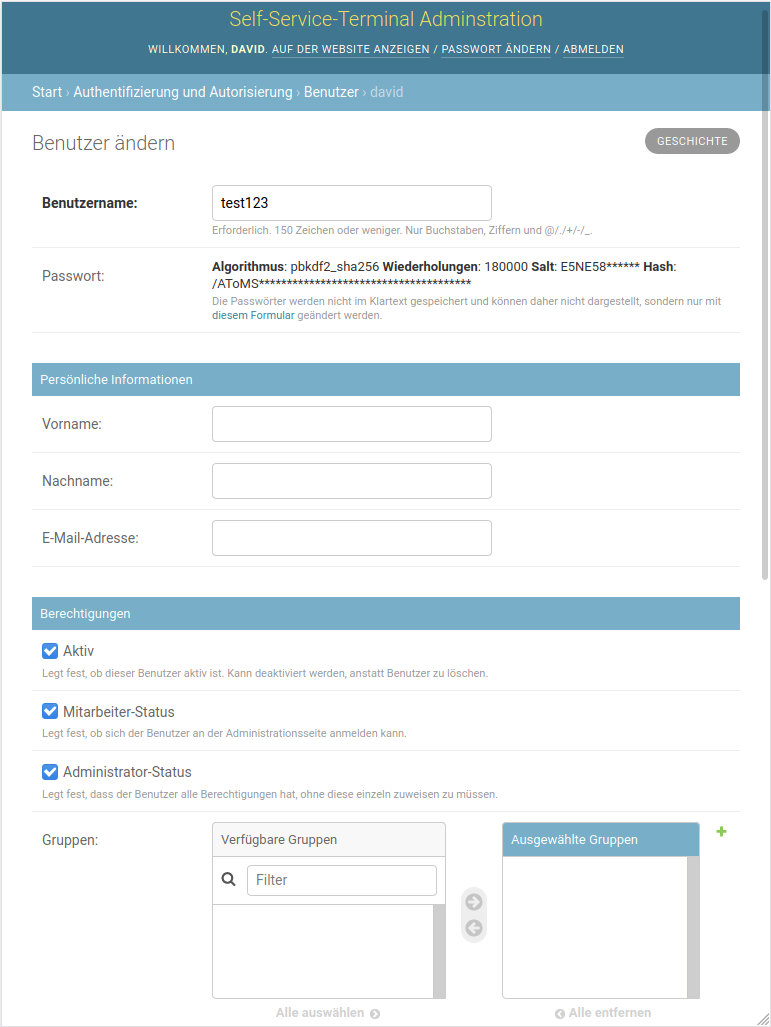
\includegraphics[width=7cm , height=10cm]{Bilder/AdminBenutzer1.png}
    \caption[Startseite des Self-Service-Terminals]{Benutzer-Einstellungen (1)}
    \label{fig:SSTBenutzer1}
\end{figure}

\begin{figure}[htp]
    \centering
    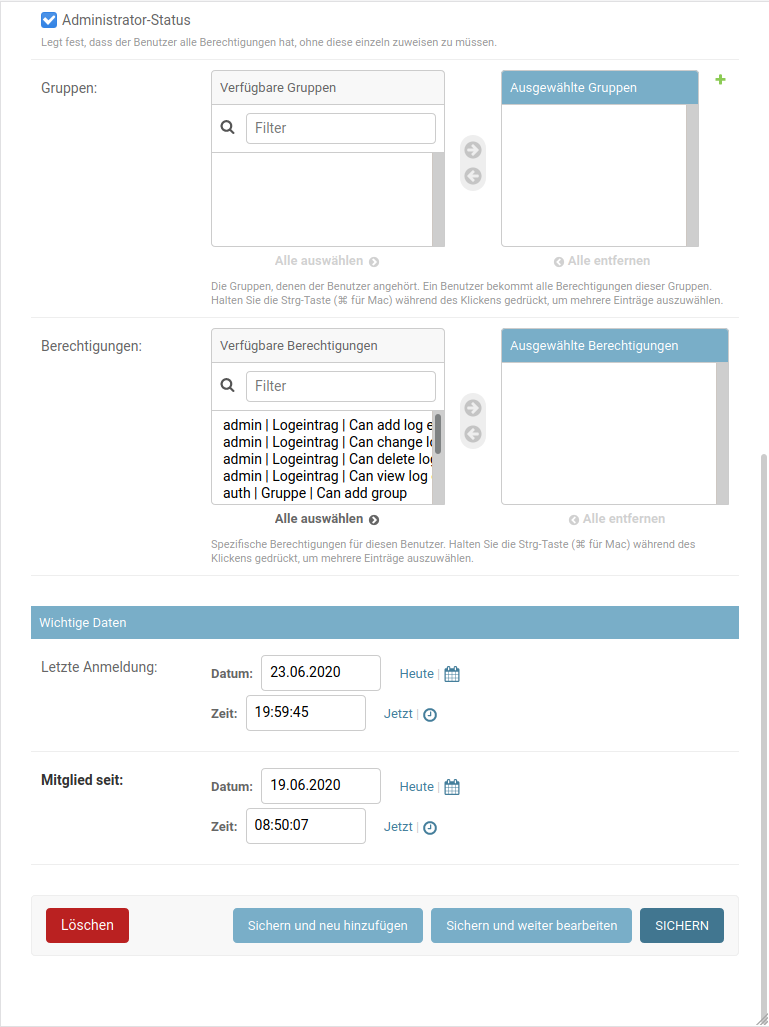
\includegraphics[width=7cm , height=10cm]{Bilder/AdminBenutzer2.png}
    \caption[Startseite des Self-Service-Terminals]{Benutzer-Einstellungen (2)}
    \label{fig:SSTBenutzer2}
\end{figure}

\newpage

\subsubsection{Gruppen} Es können Benutzergruppen angelegt und gelöscht werden. Mit diesen Benutzergruppen können beispielsweise Berechtigungen einfacher administriert werden (Abbildung 2).

\begin{figure}[htp]
    \centering
    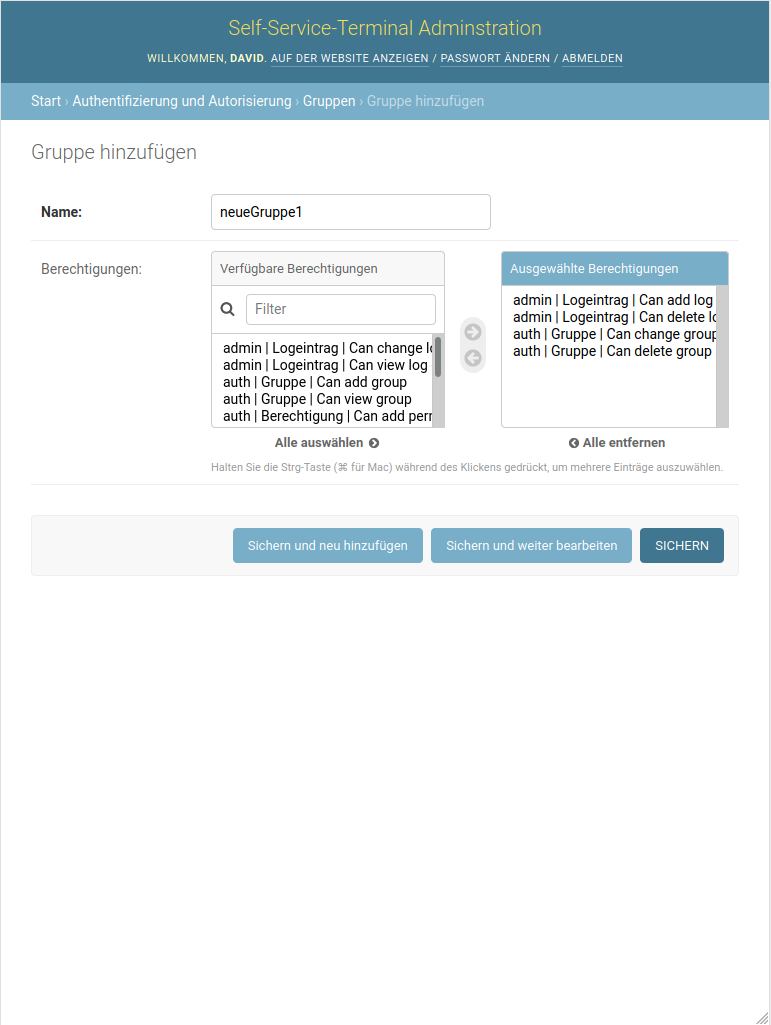
\includegraphics[width=7cm , height=10cm]{Bilder/AdminGruppe.png}
    \caption[Startseite des Self-Service-Terminals]{Gruppen-Einstellungen}
    \label{fig:SSTGruppe}
\end{figure}

\newpage

\subsubsection{Einstellungen} Es können Einstellungen-Objekte angelegt werden. Einstellungen haben einen Titel, eine Beschreibung sowie Farbeinstellungen für: Kopfleiste, Überschriften, Texte, Buttons und den Zurück-Button (Abbildung 3). Außerdem können zwei Logos hochgeladen werden. Werden die Farbeinstellungen leer gelassen, wird das Grüne Default-Theme angezeigt. Der Titel der Einstellungen muss auf \glqq settings\grqq{} gesetzt werden, damit sie vom System verarbeitet werden. Ist kein Einstellungs-Objekt gespeichert, ist das System nicht funktions fähig.

\begin{figure}[htp]
    \centering
    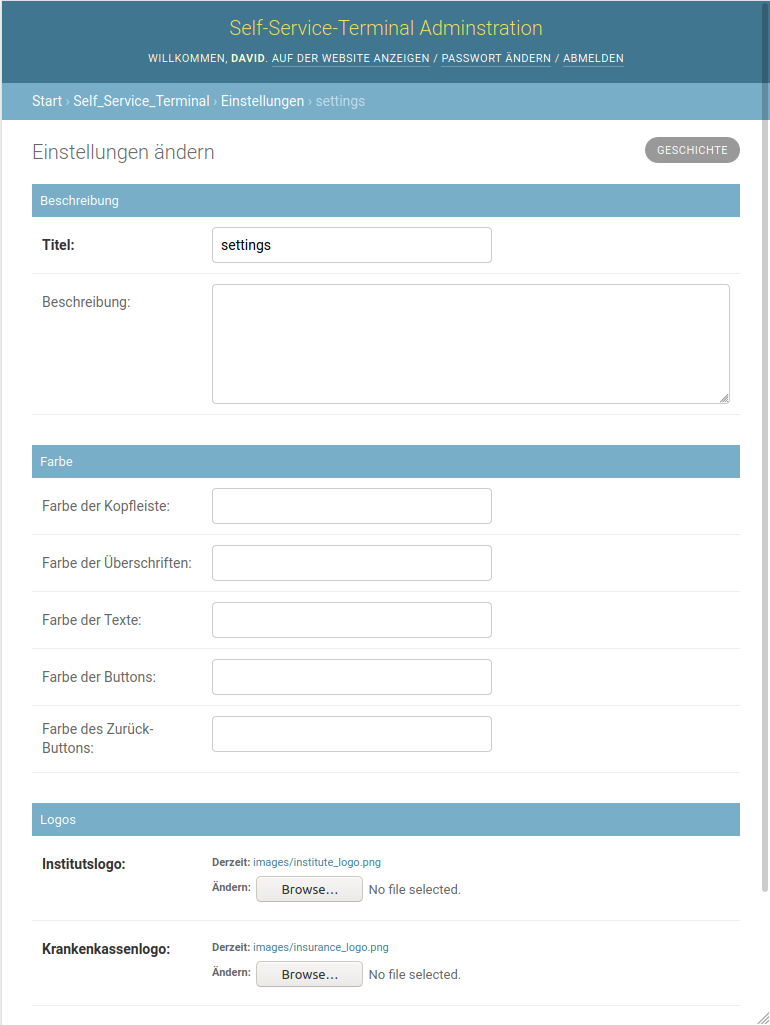
\includegraphics[width=7cm , height=10cm]{Bilder/AdminEinstellungen.png}
    \caption[Startseite des Self-Service-Terminals]{Frontend-Einstellungen}
    \label{fig:SSTAdminFrontend}
\end{figure}

\newpage

\subsubsection{Formulare} Formulare können hinzugefügt und gelöscht werden. Formulare haben ein Eltern-Menü indem sie angezeigt werden, außerdem einem Titel, eine Beschreibung und die zugehörige PDF-Datei (Abbildung 4).

\begin{figure}[htp]
    \centering
    \includegraphics[width=7cm , height=10cm]{Bilder/AdminFormularHinzufügen.png}
    \caption[Startseite des Self-Service-Terminals]{Formular-Einstellungen}
    \label{fig:SSTAdminFormular}
\end{figure}

\newpage

\subsubsection{Menüs} Menüs können hinzugefügt und gelöscht werden. Menüs haben ein Eltern-Menü um eine  Baumstruktur zu erzeugen, außerdem einen Titel und eine Beschreibung. Einem Menü können Submenüs und Formulare zugewiesen werden (Abbildung 5).

\begin{figure}[htp]
    \centering
    \includegraphics[width=7cm , height=10cm]{Bilder/AdminMenüs.png}
    \caption[Startseite des Self-Service-Terminals]{Menü-Einstellungen}
    \label{fig:SSTAdminMenü}
\end{figure}

\newpage

\subsubsection{Export/Import}Einstellungen, Formulare und Menüs können zusammen mit den zugehörigen PDF-Dateien und PNG-Dateien exportiert und importiert werden. Diese Aktion kann im Einstellungs- ,Formular- oder Menü-Reiter ausgelöst werden. Die Datenbankstrukturen werden als JSON-Datei gespeichert und zusammen mit PFDs und PNGS in einem zip-Archiv im export-Ordner gespeichert. Entsprechend entstandene oder formatierte zip-Archive können im selben Aktions-Menü importiert werden, wenn sie im export-Ordner gespeichert wurden. Der export-Ordner ist im Installationsverzeichnis unter /Self-Service-Terminal/export zu finden.

\subsubsection{Verlauf} Am rechten Bildschirmrand wird ein Verlauf der auf der Administrationsseite vorgenommenen Änderungen gespeichert (Abbildung 6).

\subsubsection{Webseite anzeigen}Mit einem Klick auf die Schaltfläche \glqq Auf der Webseite anzeigen\grqq{} (Abbildung 6) wird dem Nutzer die Startseite des Self-Service-Terminal angezeigt.

\subsubsection{Passwort ändern} Mit einem Klick auf die Schaltfläche \glqq Passwort ändern\grqq{} (Abbildung 6) wird der Nutzer auf eine Seite zum ändern des Passworts weitergeleitet.

\subsubsection{Abmelden} Mit einem Klick auf die Schaltfläche \glqq Abmelden\grqq{} (Abbildung 6) wird der Nutzer abgemeldet.

\begin{figure}[htp]
    \centering
    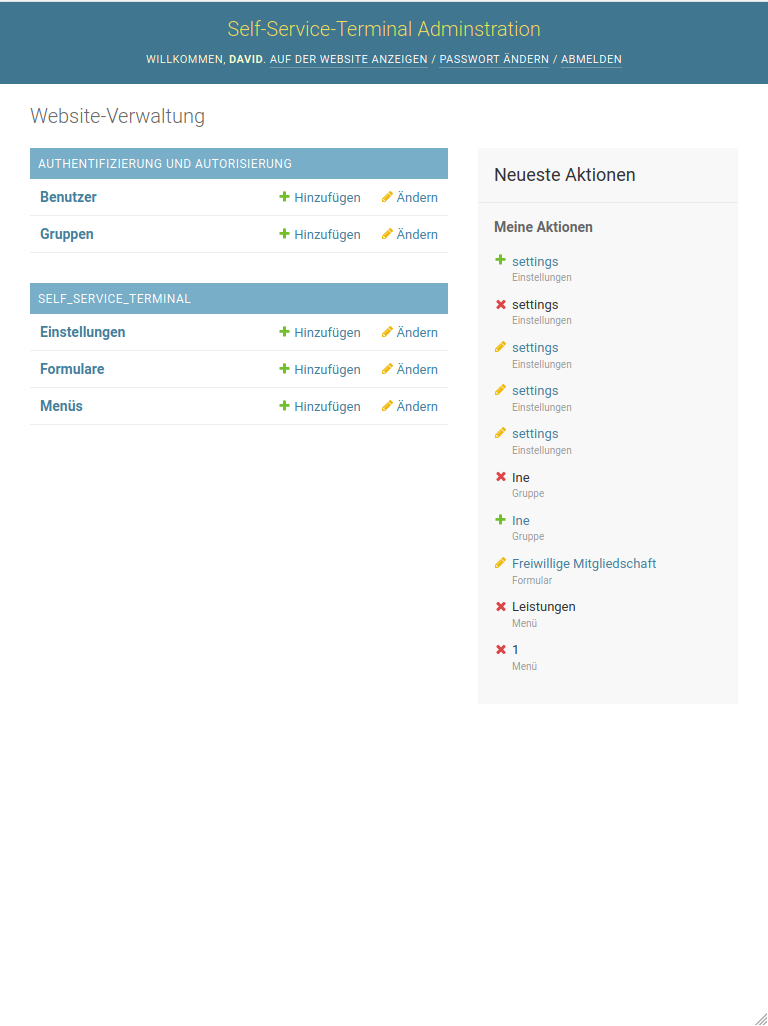
\includegraphics[width=7cm , height=10cm]{Bilder/AdminSeite.png}
    \caption[Startseite des Self-Service-Terminals]{Admin-Seite}
    \label{fig:SSTAdminSeite}
\end{figure}

\newpage

\subsection{Kundensicht}


\subsubsection{Startseite} Die Startseite (Abbildung 7) ist der Ausgangspunkt der Navigation durch die Menüstruktur des Self-Service-Terminals. Mit einem Klick auf die Schaltfläche \glqq Startseite\grqq{} in der rechten oberen Ecke der Benutzeroberfläche kann jederzeit zur Startseite zurückgekehrt werden.

\begin{figure}[htp]
    \centering
    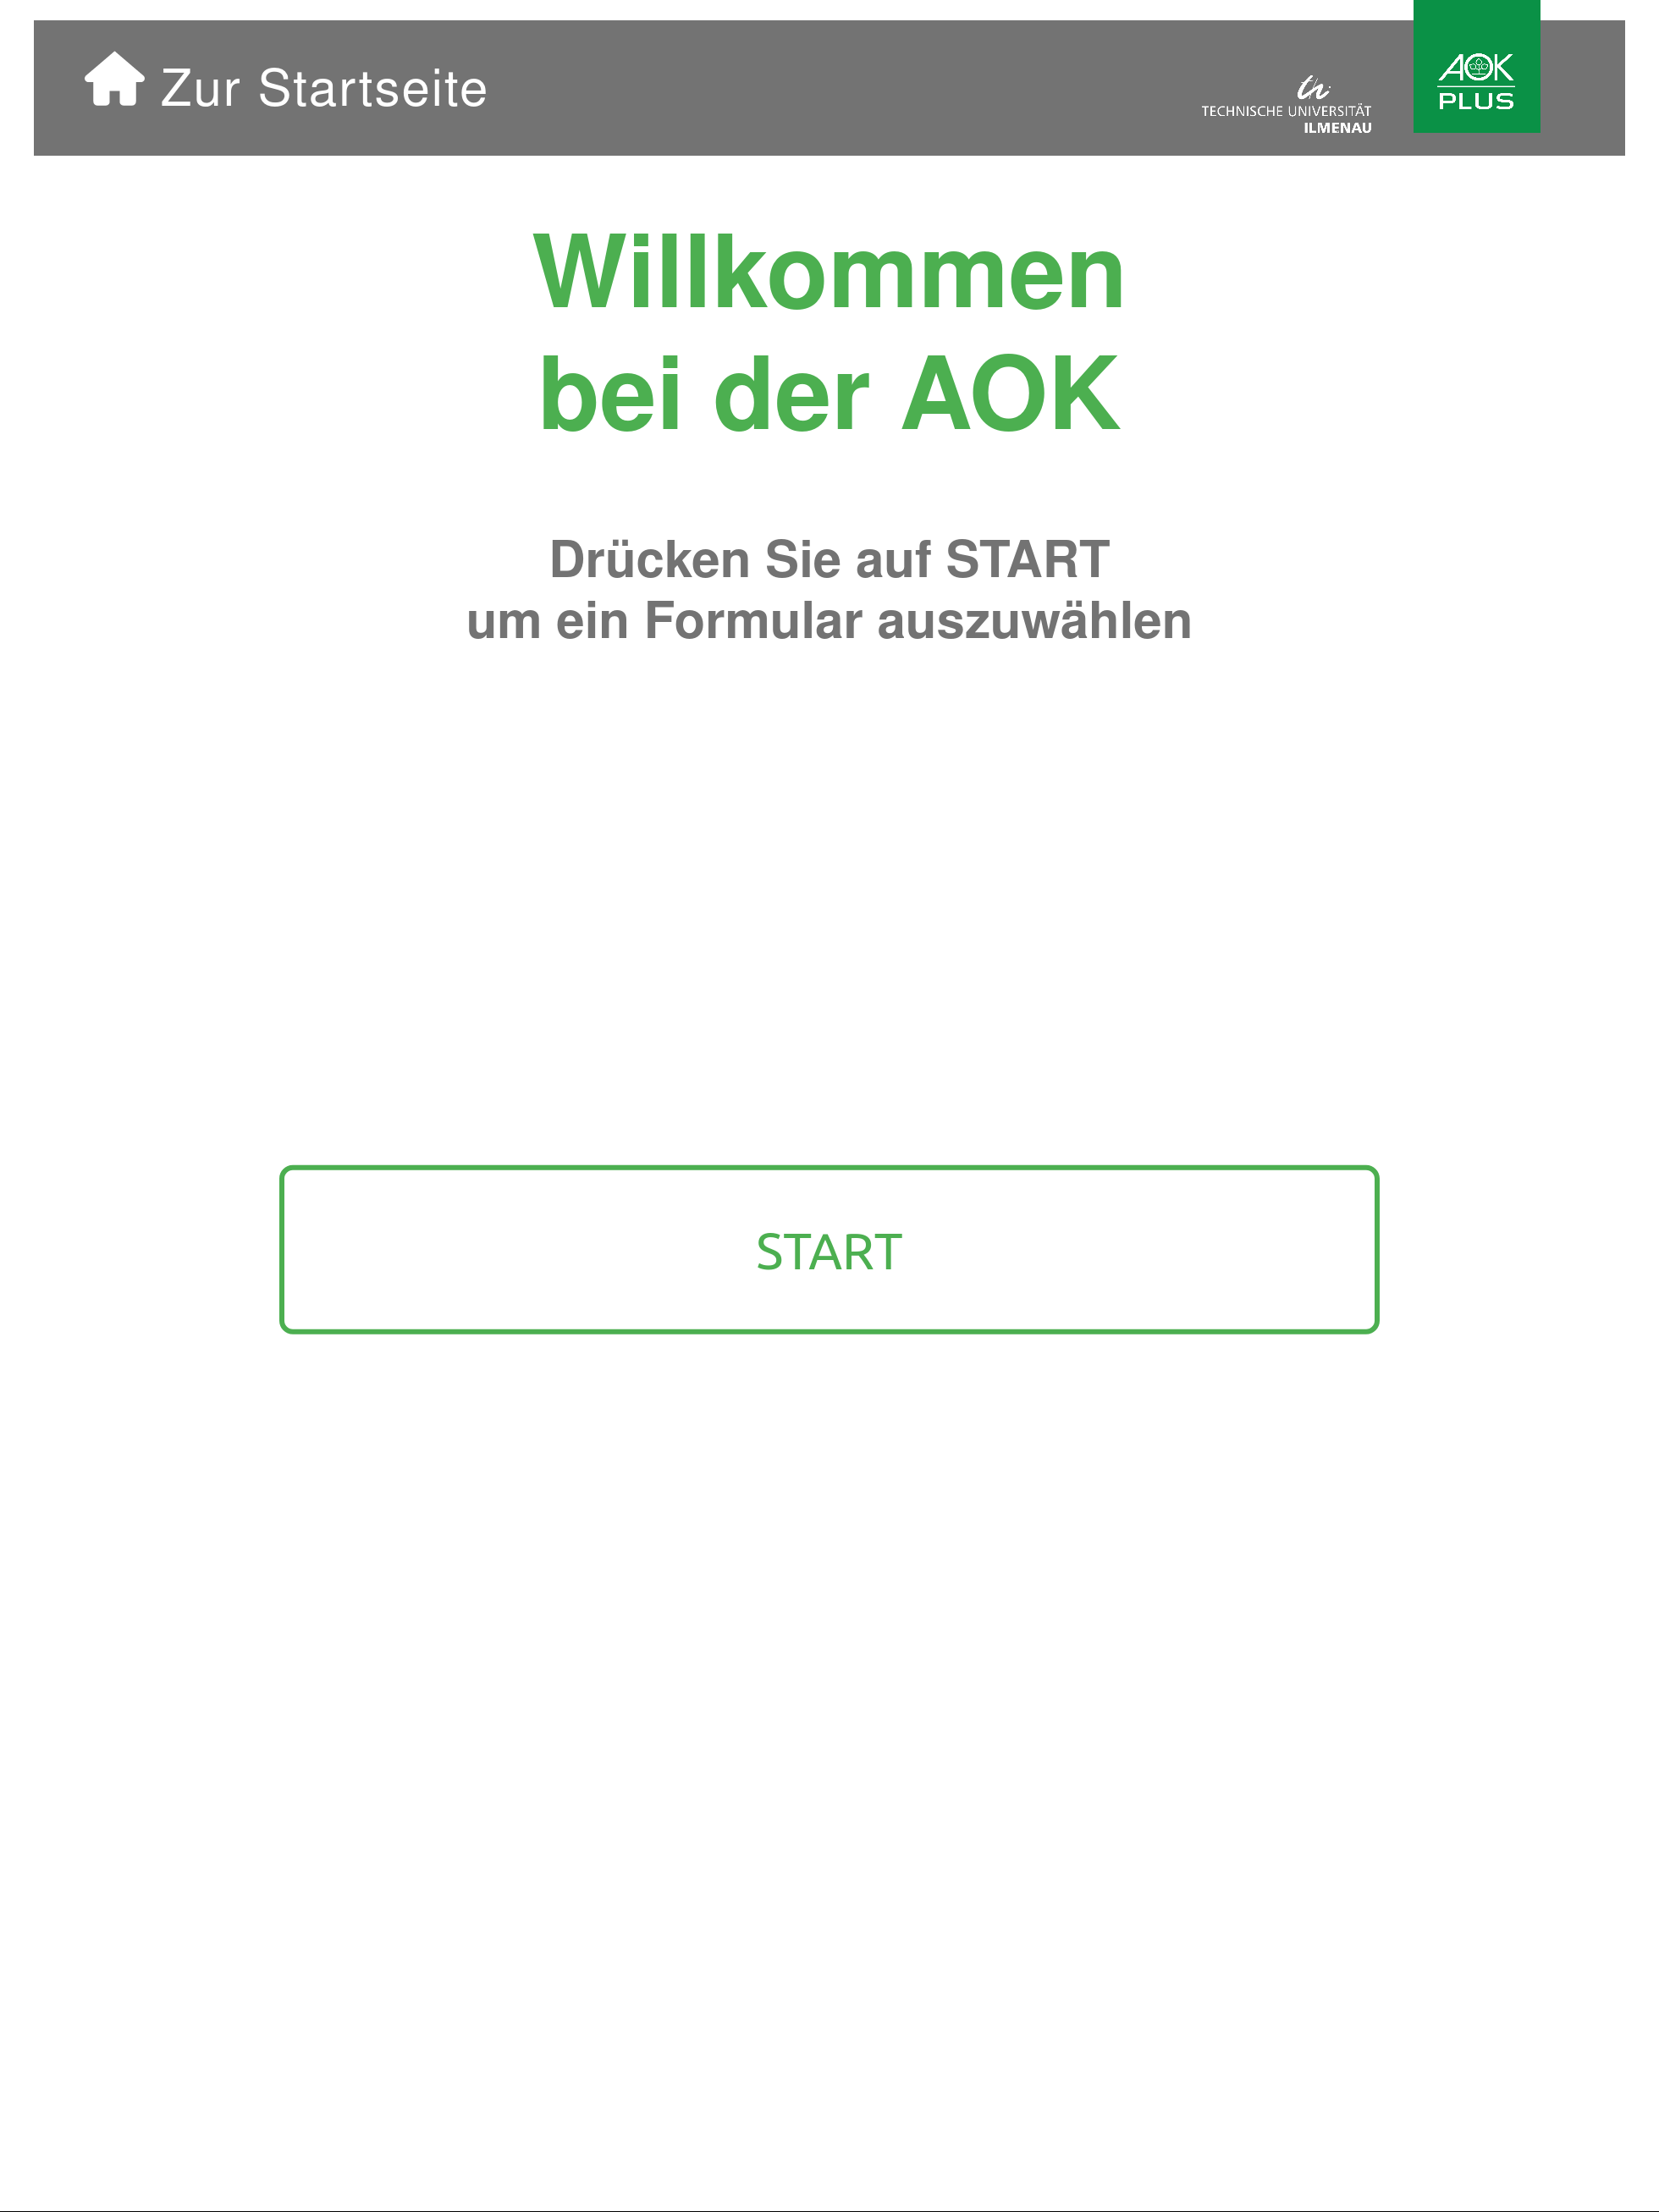
\includegraphics[width=7cm , height=10cm]{Bilder/Startseite.png}
    \caption[Startseite des Self-Service-Terminals]{Startseite des Self-Service-Terminals}
    \label{fig:SSTStart}
\end{figure}

\newpage

\subsubsection{Menüs}Menüs (Abbildung 8) enthalten Submenüs oder Formulare, welche als Buttons dargestellt werden. Formular-Buttons sind dabei mit einem Formular-Icon gekennzeichnet (Abbildung 9). Über die Buttons kann in Submenüs oder Formulare gewechselt werden. Über einen Klick auf den \glqq zurück\grqq{} Button kann man zum vorherigen Menü zurückkehren.

\begin{figure}[htp]
    \centering
    \includegraphics[width=7cm , height=10cm]{Bilder/Menü1.png}
    \caption[Startseite des Self-Service-Terminals]{Menü mit Submenüs}
    \label{fig:SSTMenüSubmenü}
\end{figure}

\begin{figure}[htp]
    \centering
    \includegraphics[width=7cm , height=10cm]{Bilder/Menü2.png}
    \caption[Startseite des Self-Service-Terminals]{Menü mit Formularen}
    \label{fig:SSTMenüFormulare}
\end{figure}

\newpage

\subsubsection{Pagination} Pagination ist eine Funtkion welche greift, wenn mehr als fünf Submenüs oder Formulare in einem Menü angezeigt werden sollen. In diesem Fall werden weitere Seiten des Menüs erstellt, welche nach einem Klick auf die Schaltfläche \glqq weitere Einträge\grqq{} angezeigt werden. Wie viele Seiten das so erweiterte Menü umfasst, wird direkt unter den Buttons angezeigt (Abbildung 10).

\begin{figure}[htp]
    \centering
    \includegraphics[width=7cm , height=10cm]{Bilder/Menü3.png}
    \caption[Startseite des Self-Service-Terminals]{Menü mit mehr als fünf Einträgen}
    \label{fig:SSTMenüPagination}
\end{figure}

\newpage

\subsubsection{Formulare}Wird ein Formular angeklickt, öffnet sich die Formular-Ansicht. Hier stehen 3 Optionen zur weiteren Navigation zur Verfügung. \glqq Vorschau\grqq{}, \glqq Drucken\grqq{} und \glqq zurück\grqq{} (Abbildung 11).

\begin{figure}[htp]
    \centering
    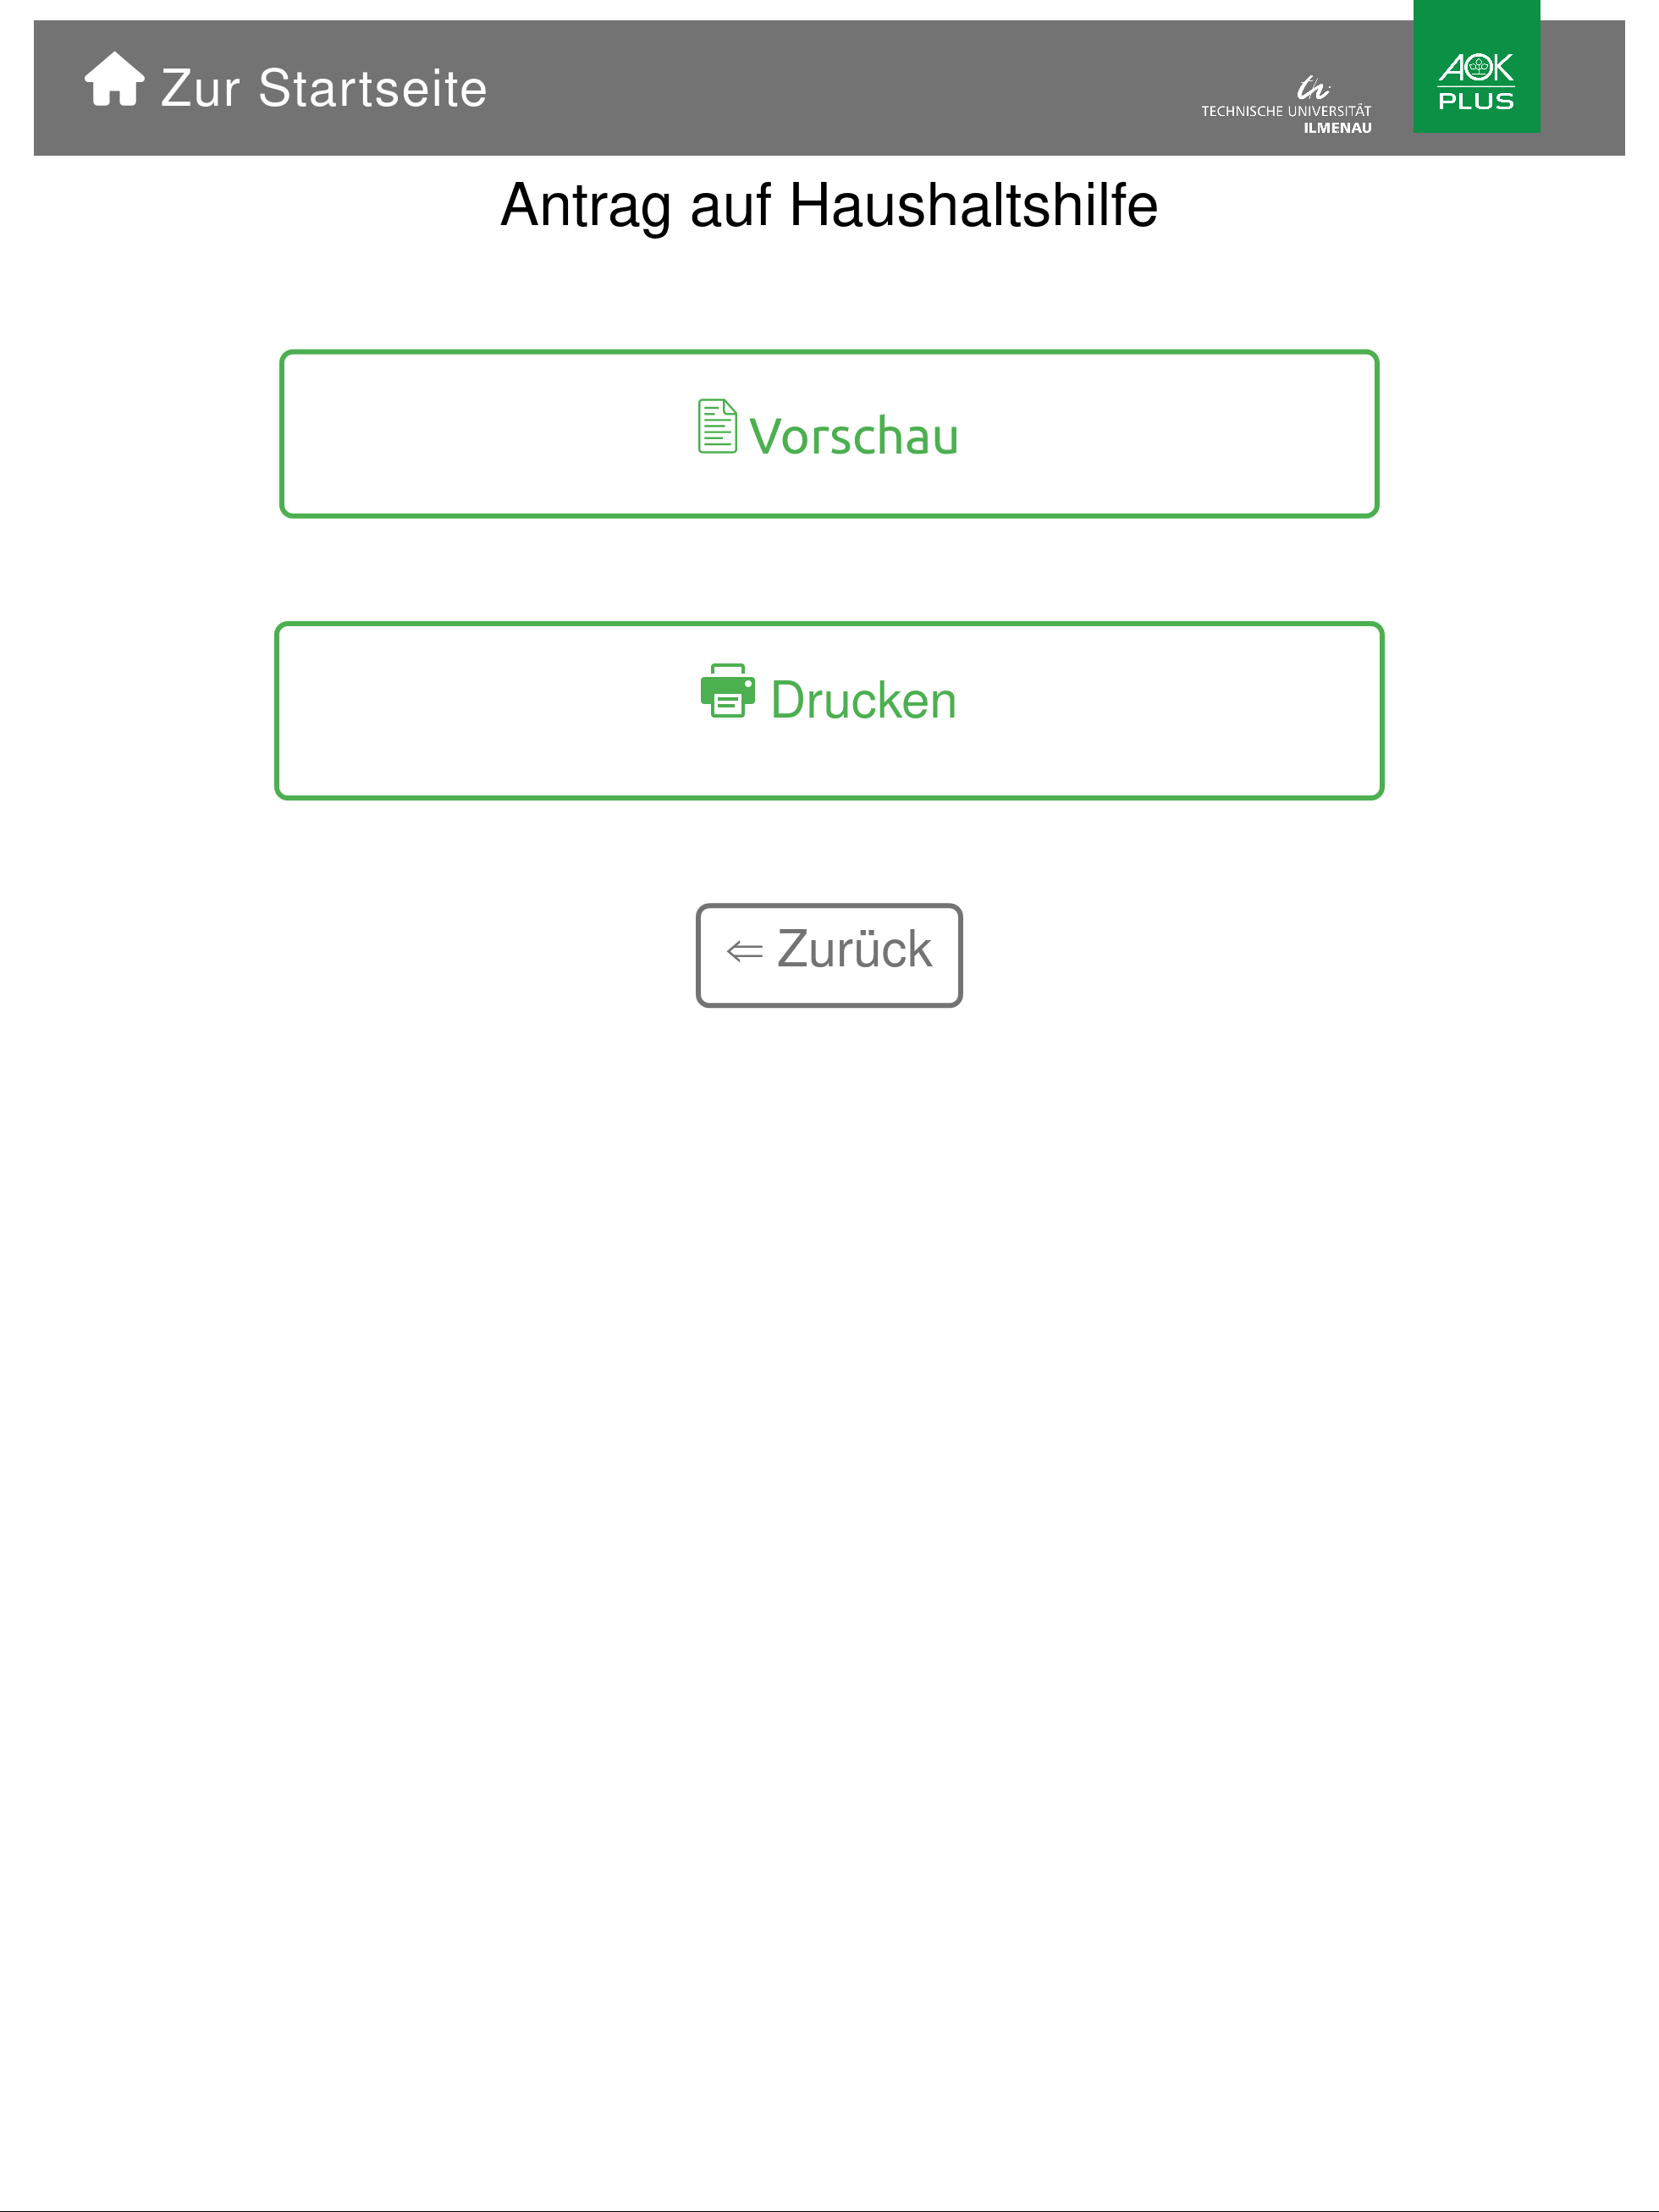
\includegraphics[width=7cm , height=10cm]{Bilder/Formular1.png}
    \caption[Startseite des Self-Service-Terminals]{Formular-Ansicht}
    \label{fig:SSTFormular}
\end{figure}

\subsubsection{Vorschau} Bei einem Klick auf den Button \glqq Vorschau\grqq{} wird eine Bilddatei des hinterlegten Formular-PDFs erzeugt und angezeigt.

\newpage

\subsubsection{Drucken} Bei einem Klick auf den Button \glqq Drucken\grqq{} wird der lp-Befehl an den Server übermittelt und der http-Code: 200 zurückgegeben. Im Anschluss wird eine Ladeanimation angezeigt um dem Nutzer ein visuelles Feedback über den Druckvorgang zu bieten (Abbildung 12).

\begin{figure}[htp]
    \centering
    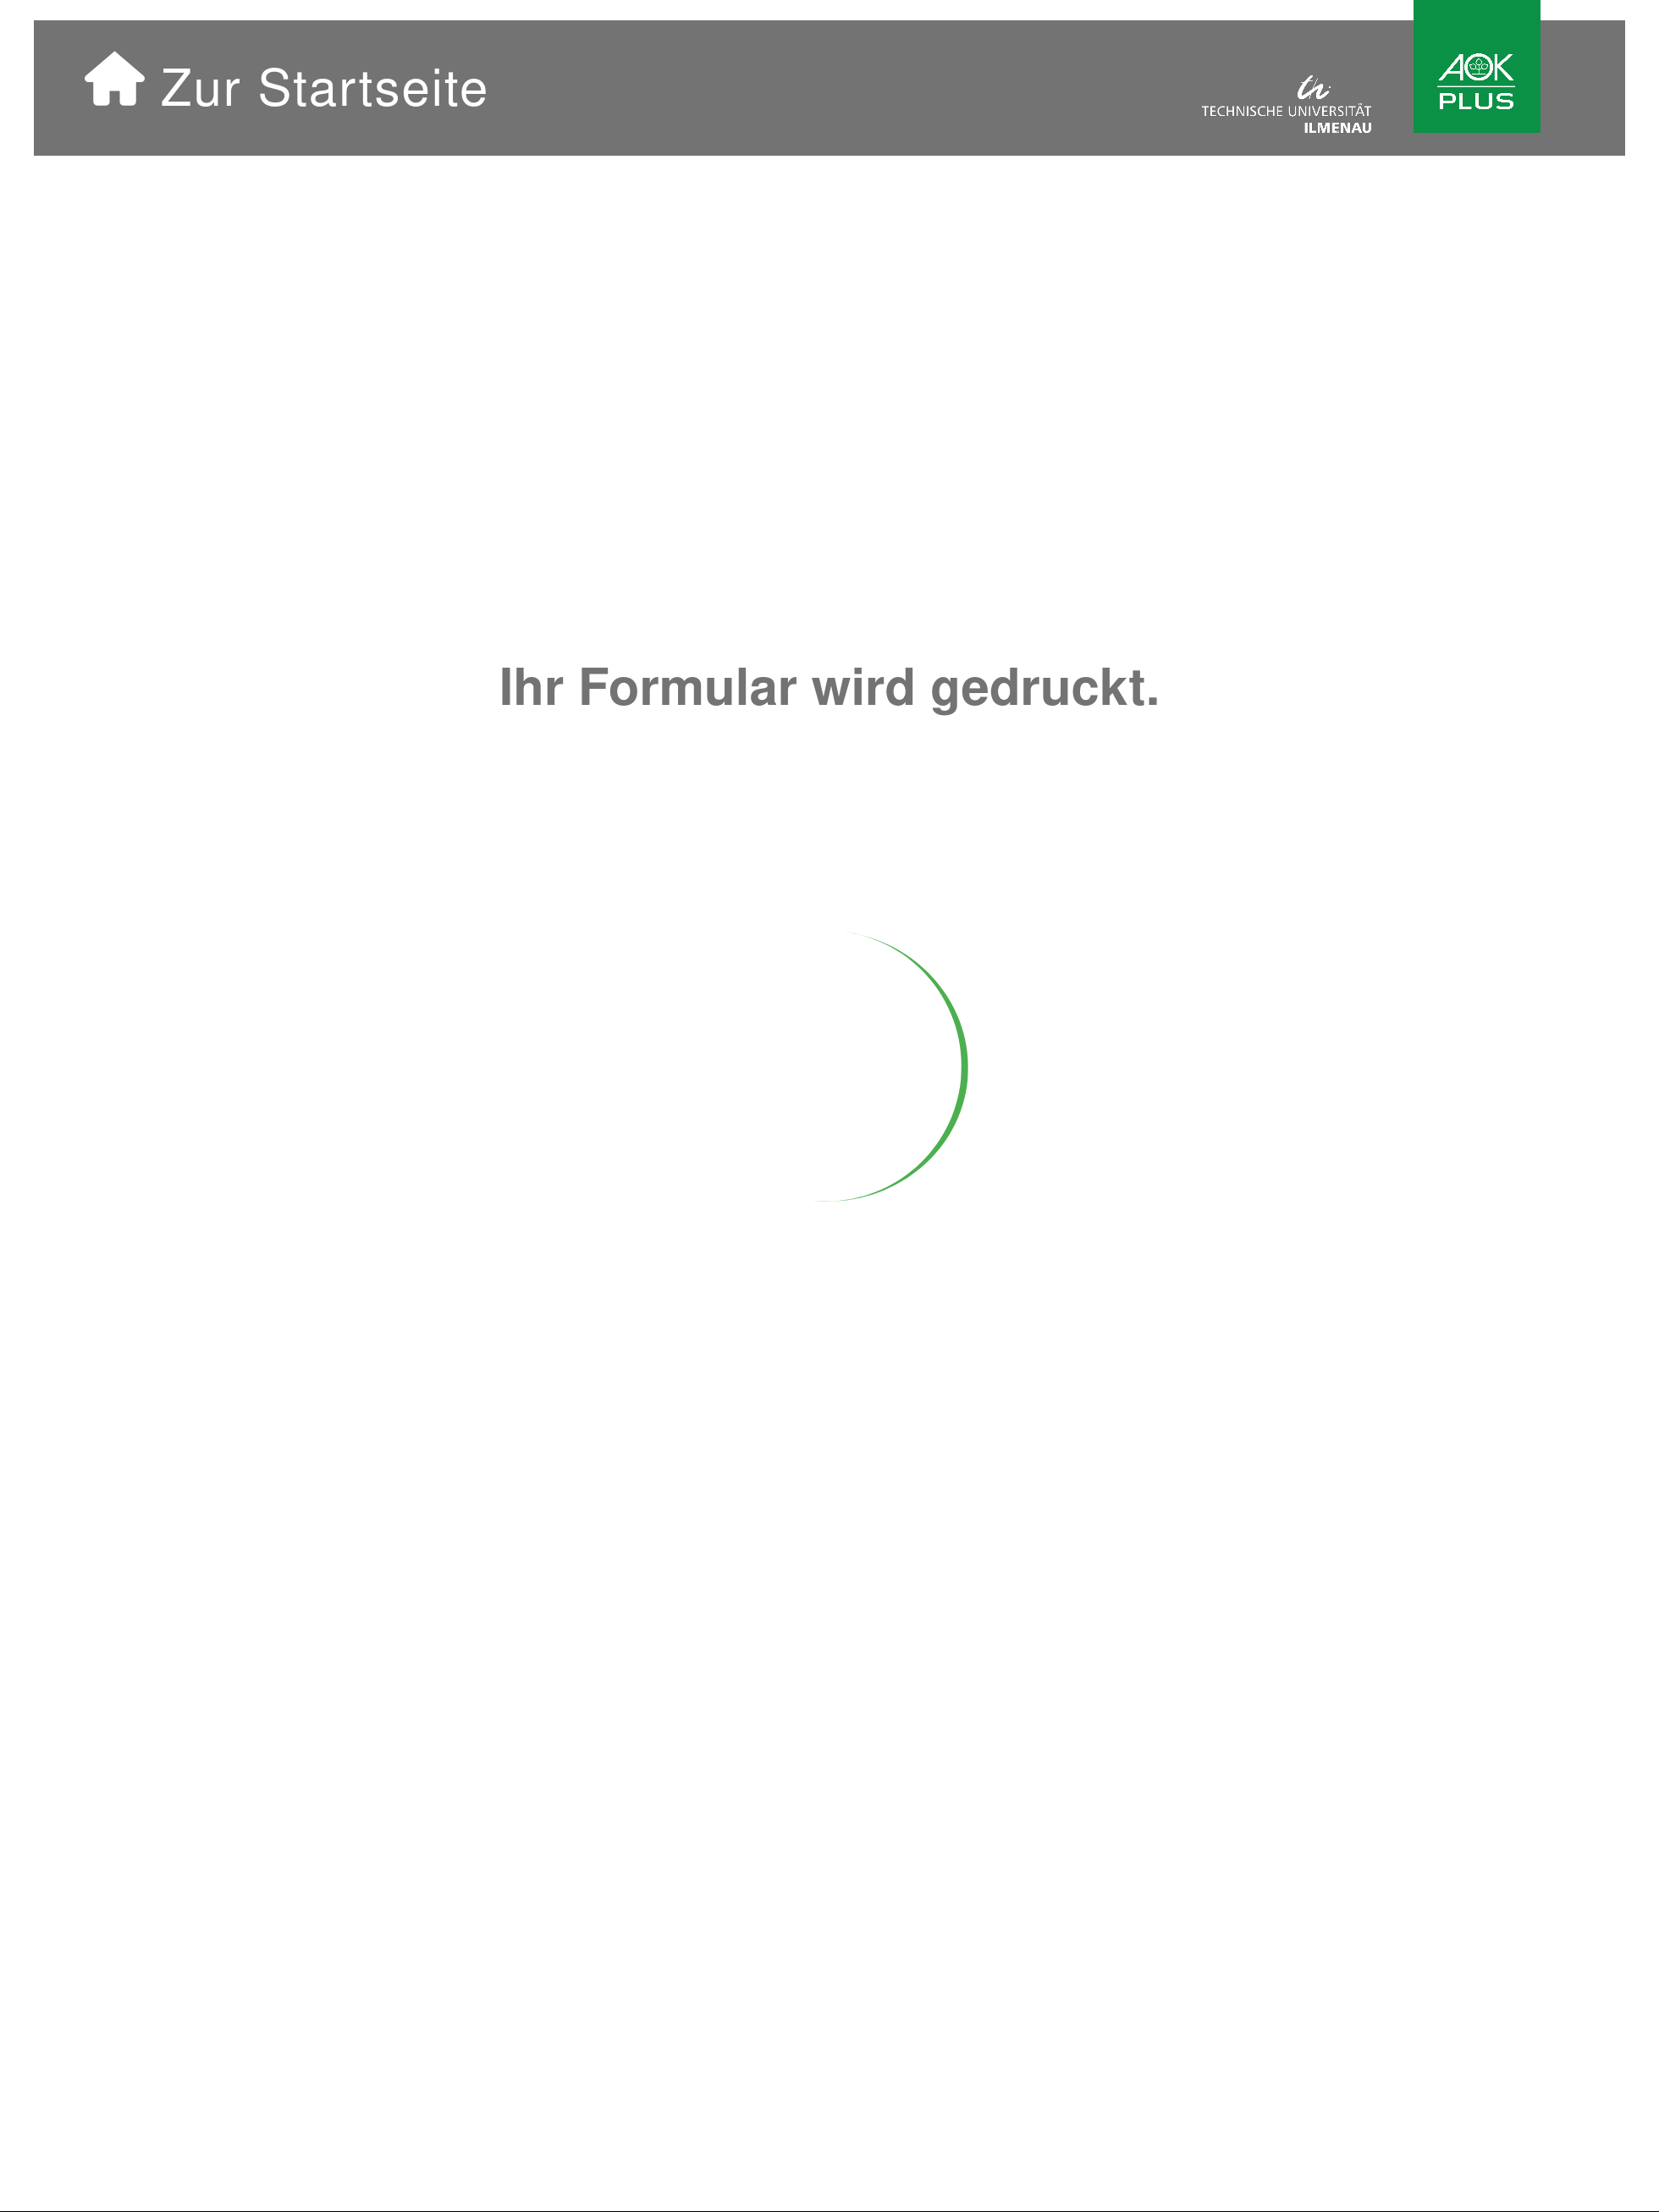
\includegraphics[width=7cm , height=10cm]{Bilder/Drucken.png}
    \caption[Startseite des Self-Service-Terminals]{Druckanimation}
    \label{fig:SSTDrucken}
\end{figure}

\subsubsection{Weiterleitung} Registriert das Self-Service-Terminal für mehr als 120 Sekunden keine Eingaben, setzt es sich auf die Startseite zurück. Gleiches passiert, nachdem ein Druckvorgang abgeschlossen wurde.

\newpage

\subsection{Systemfehler:}
Wurde der Server des Self-Service-Terminal nach der Installationsanleitung konfiguriert, startet und initialisiert er die Anwendung nach einem Neustart automatisch neu. Treten Systemfehler auf, oder ist das Self-Service-Terminal nicht erreichbar, starten Sie den Server neu und warten sie danach einige Sekunden. Sollte der Fehler auch nach einem Neustart noch bestehen, wenden Sie sich an folgende Aufzählung.
Im folgenden Erläutern wir einige Fehler, welche durch eine falsche Bedienung auftreten können, wie Sie zu erkennen und wie zu beheben sind.

\begin{itemize}
    \item Fehler: Fehlercode \textbf{Terminal\_Settings mathing query does not exist} bei Aufruf der Kundensicht.\par
    Es wurde kein Einstellungs-Objekt in der Admin-Seite festgelegt. Erstellen Sie ein Einstellungs-Objekt mit dem Titel \glqq settings\grqq{}.
    \item Fehler: Nach einem Klick auf \glqq Vorschau\grqq{} in der Formular-Ansicht wird nur eine weiße Seite angezeigt.\par
    Dem angelegten Formular wurde keine PDF-Datei zugeordnet. Laden Sie das passende PDF in den Formular Eintrag auf der Admin-Seite hoch.
    \item Fehler: Ein Klick auf die \glqq Drucken\grqq{} Schaltfläche löst keinen Druckvorgang aus, die Druckertreiber wurden aber installiert und CUPS nach der Anleitung konfiguriert\par
    Der Dateiname der PDF im files-Ordner (self-service-terminal/files) stimmt nicht mit dem Dateinamen in der Datenbank überein. Ändern Sie den Dateinamen auf den Wert, welcher in den Formular-Einstellungen auf der Admin-Seite eingestellt wurde.
\end{itemize}